%\documentclass[xcolor=dvipsnames,10pt,handout]{beamer}
% ,handout
\documentclass[9pt]{beamer}
\usepackage{etex}

%\usepackage[francais]{babel}
\usepackage[utf8]{inputenc}
\usepackage{graphicx,pstricks,pst-node,pst-plot}
\usepackage{pxfonts} %concrete,pxfonts
\usepackage{charter} %mathptmx, newcent, charter
\usepackage[mathscr]{eucal}
\usepackage{mathtools} 
\usepackage{multirow,epsfig}
\usepackage{pgf,pgflibraryshapes,pgflibraryarrows,tikz}  % old version
\usepackage{fancybox}
\usepackage{amsmath,amssymb,amsfonts,amsbsy,ifthen,rotate}
\usepackage{tabularx}
\usepackage{colortbl,xcolor}
\usepackage{setspace}
\usepackage{natbib}
\usepackage{tabularx,multirow}
\usepackage{slashbox}
\usepackage{graphicx}
\graphicspath{{../Pics/}, {../Pics/kriging_illustration/}, {../Pics/kriging_ex/}, {../Pics/random_process/}, {../Pics/cov/}, {../Pics/enrich_ED/}}

\newcommand{\altx}{\usebeamercolor[fg]{alerted text}}
\newcommand{\titx}{\usebeamercolor[fg]{subtitle}}

\newcommand{\absolute}[1]{| #1 |}
\newcommand{\Variance}[2]{\mathbb{V}\text{ar}_{#1}\left[ #2 \right])}
\newcommand{\Expectation}[2]{\mathbb{E}_{#1}\left[ #2 \right]}
\newcommand{\Prob}[2]{\mathbb{P}_{#1}\left[ #2 \right]}
\newcommand{\N}[2]{\mathcal{N}\left( #1 , #2 \right)}
\newcommand{\PG}[2]{\mathrm{PG}\left( #1 , #2 \right)}
\newcommand{\VX}[1]{\mathrm{var}_X\left( #1 \right)}
\newcommand{\EX}[1]{\mathbb{E}_X\left[ #1 \right]}
\newcommand{\VZ}[1]{\mathrm{var}_Z\left( #1 \right)}
\newcommand{\covZ}[2]{\mathrm{cov}_Z\left( #1, #2 \right)}
\newcommand{\EZ}[1]{\mathbb{E}_Z\left[ #1 \right]}
\newcommand{\tX}{\tilde{X}}
\newcommand{\tx}{\tilde{x}}
\newcommand{\xnew}{x_{\mathrm{new}}}
\newcommand{\ynew}{y_{\mathrm{new}}}
\newcommand{\R}{\mathbb{R}}
\newcommand{\bbeta}{\boldsymbol{\beta}}
\newcommand{\aalpha}{\boldsymbol{\alpha}}
\newcommand{\nnu}{\boldsymbol{\nu}}
\newcommand{\DDelta}{\boldsymbol{\Delta}}
\newcommand{\ttheta}{\boldsymbol{\theta}}
\newcommand{\ff}{\textbf{f}}
\newcommand{\bb}{\textbf{b}}
\newcommand{\VV}{\textbf{V}}
\newcommand{\A}{\textbf{A}}
\newcommand{\RR}{\textbf{R}}
\newcommand{\rr}{\textbf{r}}
\newcommand{\z}{\textbf{z}}
\newcommand{\D}{\textbf{D}}
\newcommand{\F}{\textbf{F}}

\definecolor{colorpurple1}{rgb}{0.698,0.266,0.635}
\definecolor{colorred1}{rgb}{0.79,0,0.21}
\definecolor{colororange1}{rgb}{1,0.27,0.00}

\definecolor{cornellred}{rgb}{0.6, 0., 0.}



% Abreviations

% Symboles math
\newcommand{\bs}[1]{\boldsymbol #1}
\newcommand{\ssf}[1]{\mbox{\textsf #1}}
\newcommand{\bsf}[1]{\mbox{\textbf{\textsf #1}}}
\newcommand{\model}{\mathcal{M}}
\newcommand{\E}[1]{\mathbb{E}\left[ #1 \right]}
\newcommand{\V}[1]{\mathbb{V}\mbox{ar}\left[ #1 \right]}
\newcommand{\tr}{\textsf{T}}
\newcommand{\trinorm}{\big\|\!\big|}
\newcommand{\idx}{\boldsymbol{\alpha}}
\newcommand{\NM}{\mathbb{N}^M}
\newcommand{\RM}{\mathbb{R}^M} % math abbreviations

\newcolumntype{C}[1]{>{\centering\let\newline\\\arraybackslash\hspace{0pt}}m{#1}}

%%% First slide informations

\title[Introduction to metamodels] 
{\textcolor{orange}{ Introduction to Gaussian process metamodel - Kriging  }}

%\author[L. Le Gratiet \& G. Blatman]{L. Le Gratiet \& G. Blatman}

%institute[EDF]{EDF R\&D}

%\date\today
\date{\textcolor{orange}{\begin{flushleft} May 2020 \end{flushleft}}}


%%% General options

\setbeamercolor{frametitle}{fg=orange}
\setbeamerfont{frametitle}{size=\huge}
\setbeamercolor{alerted text}{fg=orange}
\setbeamerfont{alerted text}{series=}

% theme beamer
\usetheme{boxes}
\usecolortheme{seagull}

\mode<presentation> {
  \usetheme{boxes}
  \usecolortheme{seagull}
  \setbeamercovered{transparent}
}

%\usefonttheme[onlymath]{serif}

%\AtBeginSection[]
%{
%\setbeamertemplate{background canvas}{\pgfuseimage{section_image}}
%  \begin{frame}<beamer>
%\begin{minipage}{6cm}%
%         \textcolor{orange}{  \tableofcontents[sectionstyle=show/shaded,subsectionstyle=show/show/hide]}
%\end{minipage} 
%  \end{frame}
%\addtocounter{framenumber}{-1}
%\setbeamertemplate{background canvas}[default]
%}

%\AtBeginSubsection[]
%{
%\setbeamertemplate{background canvas}{\pgfuseimage{section_image}}
%  \begin{frame}<beamer>
%\begin{minipage}{6cm}%
%% \insertsection 
%%\vskip2em
%  \textcolor{orange}{\tableofcontents[sectionstyle=show/shaded,subsectionstyle=show/shaded/hide] }
%\end{minipage} 
%  \end{frame}
%\addtocounter{framenumber}{-1}
%\setbeamertemplate{background canvas}[default]
%}

\AtBeginSection[] {
  \begin{frame}<beamer>{Outline}
    \tableofcontents[sectionstyle=show/shaded,subsectionstyle=show/show/hide]
  \end{frame}
}

%\AtBeginSubsection[] {
%  \begin{frame}<beamer>{Outline}
%    \tableofcontents[sectionstyle=show/shaded,subsectionstyle=show/shaded/hide]
%  \end{frame}
%}

%%% Slides

\begin{document}

%% Header slide
%\part*{} % title
%\begin{frame}
%  \titlepage
%  \vspace*{-0.4cm}
 % \begin{figure}[b]
  %      \includegraphics[height=1.0cm]{../Pics/EDF.jpg}
 %   \end{figure}
%\end{frame}

\footnotesize

\pgfdeclareimage[height=1.0\paperheight, width=1.1\paperwidth]{title_image}{background_pages/title.pdf}
\pgfdeclareimage[height=1.0\paperheight, width=1.1\paperwidth]{section_image}{background_pages/section.pdf}
\setbeamertemplate{background canvas}{\pgfuseimage{title_image}}

%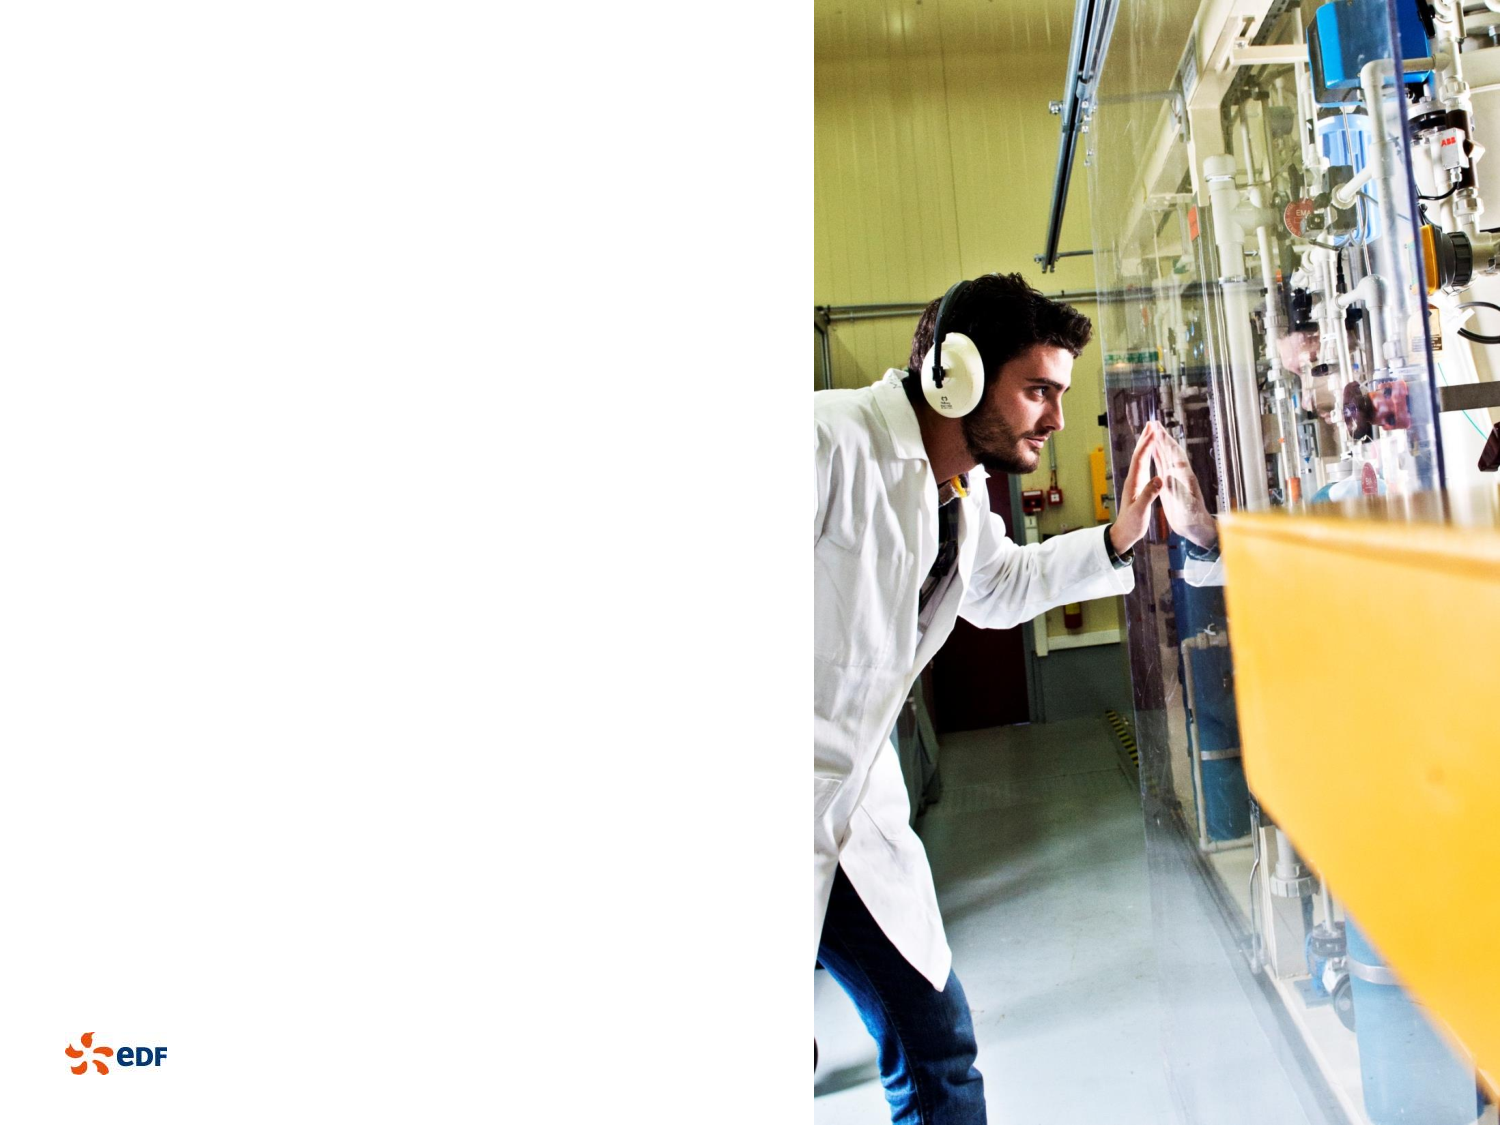
\includepdf{end.pdf}

\begin{frame}[plain]
		\vskip8ex
\begin{columns}[t]
	\begin{column}{5.5cm}
  \titlepage
 % \vspace{5ex}
   \textcolor{gray}{\tiny Copyright  EDF 2020 - Chu Mai (EDF R\&D/MMC)}
  	\end{column}
	\begin{column}{3.2cm}
	  	\end{column}
	  	\end{columns}
\end{frame}



\setbeamertemplate{background canvas}[default]


%%%%%% Table of contents page
%\setbeamertemplate{background canvas}{\pgfuseimage{section_image}}
%  \begin{frame}{Outline}
%\begin{minipage}{6cm}%
%      \tableofcontents[sectionstyle=show/show,subsectionstyle=shade/shade/shade]
%\end{minipage} 
%  \end{frame}
%\addtocounter{framenumber}{-1}
%\setbeamertemplate{background canvas}[default]
%%%%% Table of contents page

%% Body
\part*{} 
\normalsize
\setstretch{1.3}

\begin{frame}{Outline}
  \tableofcontents[sectionstyle=show/show, subsectionstyle=show/show/show]
\end{frame}

%=======================================================================================================%
\section{Random process}
%=======================================================================================================%

%=======================================================================================================%
\begin{frame}[t]{Random variable and random vector}

{\bf Random variable}: variable whose values depend on outcome of a random phenomenon

A random variable $X$ is a function from a set of possible outcomes $\Omega$ to a measurable space $E$:
\[
X : \Omega \to E
\]
%in which:
%\begin{itemize}
%\item $\Omega$: set of possible outcomes
%\item $E$: measurable space
%\end{itemize}

$\Omega$ being a sample space of the probability triple $(\Omega, \mathcal{F}, \mathcal{P})$  in which:
\begin{itemize}
%%\item $\Omega$: sample space of all outcomes
\item $\mathcal{F}$: set of events, each event contains zero or more outcomes
\item $\mathcal{P}$: probability measure, assigment of probability to events
\end{itemize}



Example: rolling a fair dice, outcome $\omega$, set of possible outcomes: six faces $\Omega= \{ 1, \dots, 6 \}$. Random variable $X$: $X = 1$ if $\omega \in \{ 1, 2 \}$, $X = 2$ if $\omega \in \{ 3, 4 \}$, $X = 3$ if $\omega \in \{ 5, 6 \}$. Probabilities assigned to its values $\Prob{}{X=1} = \frac{1}{3}$

{\bf Random vector}: a vector of random variables
\[
\bs{X}=(X_1,\dots,X_n)
\]

\end{frame}

%=======================================================================================================%
%\begin{frame}[t]{Random variable}
%
%\begin{itemize}
%\item Discrete: coin toss, dice roll. $\Omega = \{ head, tail \}$, $Y = 1$ when $\omega = head$, $Y = 0$ when $\omega = tail$
%\item Continuous: height of people on earth
%\end{itemize}uch that Z (x) is a random
%variable. Alternatively a stochastic
%process is a functio
%
%
%Probability distribution function
%
%Cumulative distribution function
%
%Random vector: a vector of random variables
%
%\[
%\bs{X} = (X_1, \dots , X_n)
%\]
%
%\end{frame}

%=======================================================================================================%
\begin{frame}[t]{Random process}

{\bf Random process} Y: set of random variables indexed by $x$ and defined in the probability space $(\Omega, \mathcal{F}, \mathcal{P})$
\[
Y: \Omega \, x \, \mathcal{D} \to E
\]
$\mathcal{D} \subset \mathbb{R}^d$: space of indices (e.g. spatial, temporal domains)

\begin{itemize}
\item At a given point $x_0 \in \mathcal{D}$, $Y(\omega, x_0)$ is a random variable.
\item With a given random event $\omega_0 \in \Omega$ and index $x \in \mathcal{D}$, one obtains a function (a.k.a realisation, trajectory):
\[
y(\omega_0, x): x \in \mathcal{D}  \to \mathbb{R} 
\]
\end{itemize}

\begin{center}
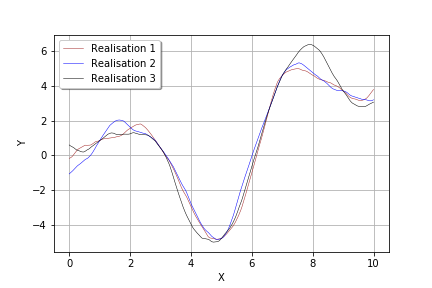
\includegraphics[width=0.45\linewidth]{realisations.png}
\end{center}

\end{frame}

%=======================================================================================================%
\begin{frame}[t]{Random process}

\textbf{Mean}:

\[
\mu_x = \Expectation{}{Y(x)}
\]

%if $mu_x$ exists for all $x \in \mathcal{D}$: 
\textbf{Covariance}:

\[
C(x,x') \coloneqq C( Y(x), Y(x') ) = \Expectation{}{ ( Y(x) - m_x ) ( Y(x') - m_{x'} ) }
\]

\textbf{Stationary random process}: the covariance function $C(x,x')$ depends only on $\tau = x - x'$, not on the position in the space

\[
C(x, x') = C(x-x') = C(\tau)
\]

\textit{\textbf{Gaussian process}}: the random process $Y: \Omega \, x \, \mathcal{D} \to E$ is called a gaussian process if every finite collection of random variables is a Gaussian random vector (i.e. has a multi-variate normal distribution)

\begin{center}
$\forall k, \forall \{x_1, \dots , x_k \} \in \mathcal{D}^k$, $\{ Y(x_1), \dots , Y(x_k) \} \sim \mathcal{N}( \bs{\mu}, \bs{C} ); \, \bs{C}_{ij} = C(x_i, x_j)$ 
\end{center}


\end{frame}

%=======================================================================================================%
\begin{frame}[t]{Covariance function of a stationary random process}

Global form of a unidimensional covariance function (Schlather 2009):
\[
C(x, x') = C_0 + \upsilon \, \rho \left( \frac{\absolute{x-x'}}{l} \right)
\]

\begin{itemize}
\item $C_0$: nugget effect
\item $\upsilon$: constant variance of the random process
\item $l$: correlation length
\end{itemize}

Examples of covariance functions: 
\begin{center}
\begin{tabular}{ll}
  \hline
  Kernel & Function \\
  \hline
  Mat\'{e}rn &  $C_{\nu}(\tau)  = \sigma^2 \frac{2^{1-\nu}}{\Gamma(\nu)}
 \left( \frac{\sqrt{2\nu} \absolute{\tau}}{\theta} \right)^\nu
 K_\nu \left( \frac{\sqrt{2\nu} \absolute{\tau}}{\theta} \right)$ \\
  Generalized exponential &   $C(\tau)  = \sigma^2 \exp \left( -\frac{\absolute{\tau}^\gamma}{\theta^\gamma} \right)$\\
  Squared exponential &  $C(\tau)  = \sigma^2 \exp \left( -\frac{1}{2} \frac{\absolute{\tau}^2}{\theta^2} \right)$ \\
  \hline
\end{tabular}
\end{center}

\end{frame}

%=======================================================================================================%
\begin{frame}[t]{Covariance function}

The regularity of the process is determined by the differentiability of $C(\tau)$ at $\tau = 0$.

For stationary processes, the trajectories $y(x)$ are $p$-times differentiable if $C(\tau)$ is $2p$ times differentiable at $\tau = 0$.



\begin{center}
\begin{tabular}{ll}
  \hline
  $\nu$ & Mat\'{e}rn covariance function \\
  \hline
   $\nu = 1/2 $ & $C_{1/2}(\tau) = \sigma^2 exp( - \frac{\absolute{\tau}}{\rho} )$ \\
   $\nu = 3/2 $ &   $C_{3/2}(\tau) = \sigma^2 \, (1+ \frac{\sqrt{3}\absolute{\tau}}{\rho}) \, exp( - \frac{\sqrt{3}\absolute{\tau}}{\rho} )$\\
   $\nu = 5/2 $ &  $C_{5/2}(\tau) = \sigma^2 \, (1+ \frac{\sqrt{5}\absolute{\tau}}{\rho} + \frac{5 {\absolute{\tau}}^2 }{3 \rho^2} ) \, exp( - \frac{\sqrt{5}\absolute{\tau}}{\rho} )$ \\
  \hline
\end{tabular}
\end{center}

\end{frame}

%=======================================================================================================%
\begin{frame}[t]{Covariance function}

\begin{center}
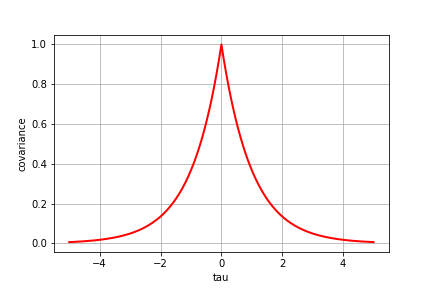
\includegraphics[width=0.48\linewidth]{cov_func_Matern_model__nu___1_2.png} 
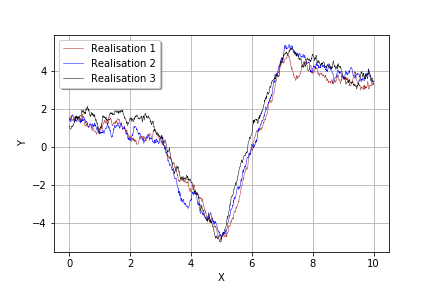
\includegraphics[width=0.48\linewidth]{realisation_Matern_model__nu___1_2.png} \\

$\nu = 1/2$
\end{center}

\begin{center}
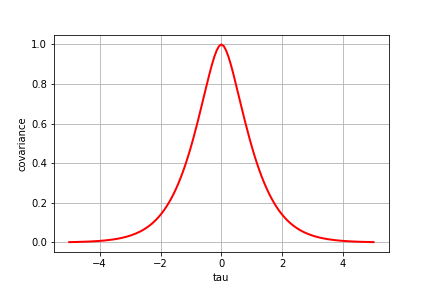
\includegraphics[width=0.48\linewidth]{cov_func_Matern_model__nu___3_2.png} 
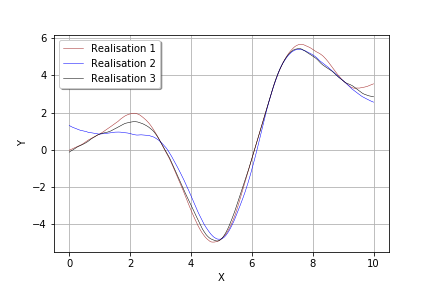
\includegraphics[width=0.48\linewidth]{realisation_Matern_model__nu___3_2.png} \\

$\nu = 3/2$

\end{center}

\end{frame}

%=======================================================================================================%
\begin{frame}[t]{Covariance function}

\begin{center}
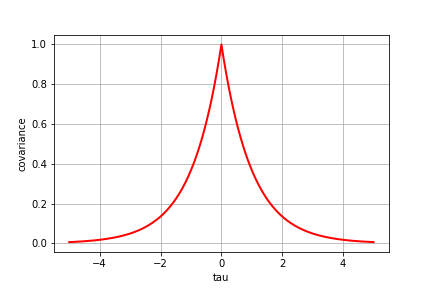
\includegraphics[width=0.48\linewidth]{cov_func_Matern_model__nu___1_2__scale___1.png} 
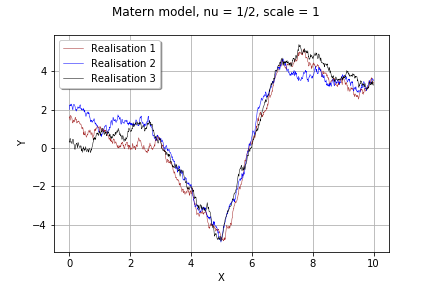
\includegraphics[width=0.48\linewidth]{realisation_Matern_model__nu___1_2__scale___1.png} \\

$\rho = 1$
\end{center}

\begin{center}
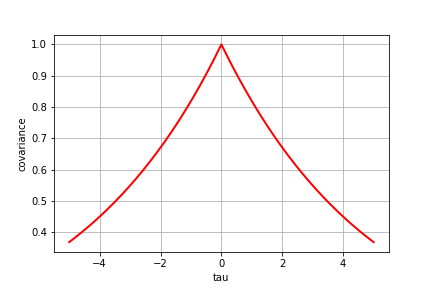
\includegraphics[width=0.48\linewidth]{cov_func_Matern_model__nu___1_2__scale___5.png} 
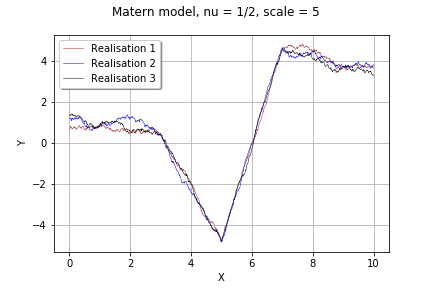
\includegraphics[width=0.48\linewidth]{realisation_Matern_model__nu___1_2__scale___5.png} \\

$\rho = 5$

\end{center}

\end{frame}

%=======================================================================================================%
\begin{frame}[t]{Covariance function}

\begin{center}
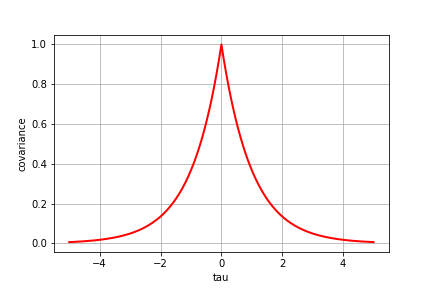
\includegraphics[width=0.48\linewidth]{cov_func_Matern_model__nu___1_2__amplitude___1.png} 
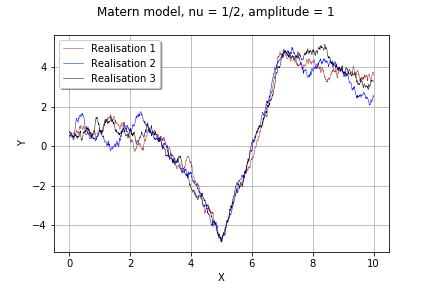
\includegraphics[width=0.48\linewidth]{realisation_Matern_model__nu___1_2__amplitude___1.png} \\

$\sigma = 1$
\end{center}

\begin{center}
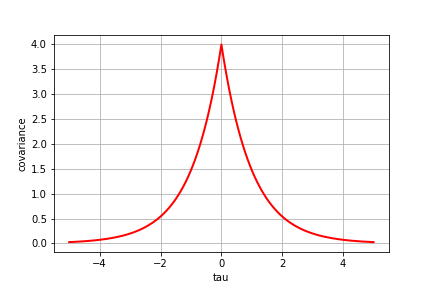
\includegraphics[width=0.48\linewidth]{cov_func_Matern_model__nu___1_2__amplitude___2.png} 
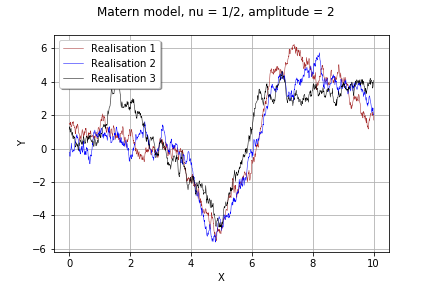
\includegraphics[width=0.48\linewidth]{realisation_Matern_model__nu___1_2__amplitude___2.png} \\

$\sigma = 2$

\end{center}

\end{frame}


\section{Gaussian process metamodel}

%=======================================================================================================%

\begin{frame}[t]{Prediction at a new point}

\begin{center}

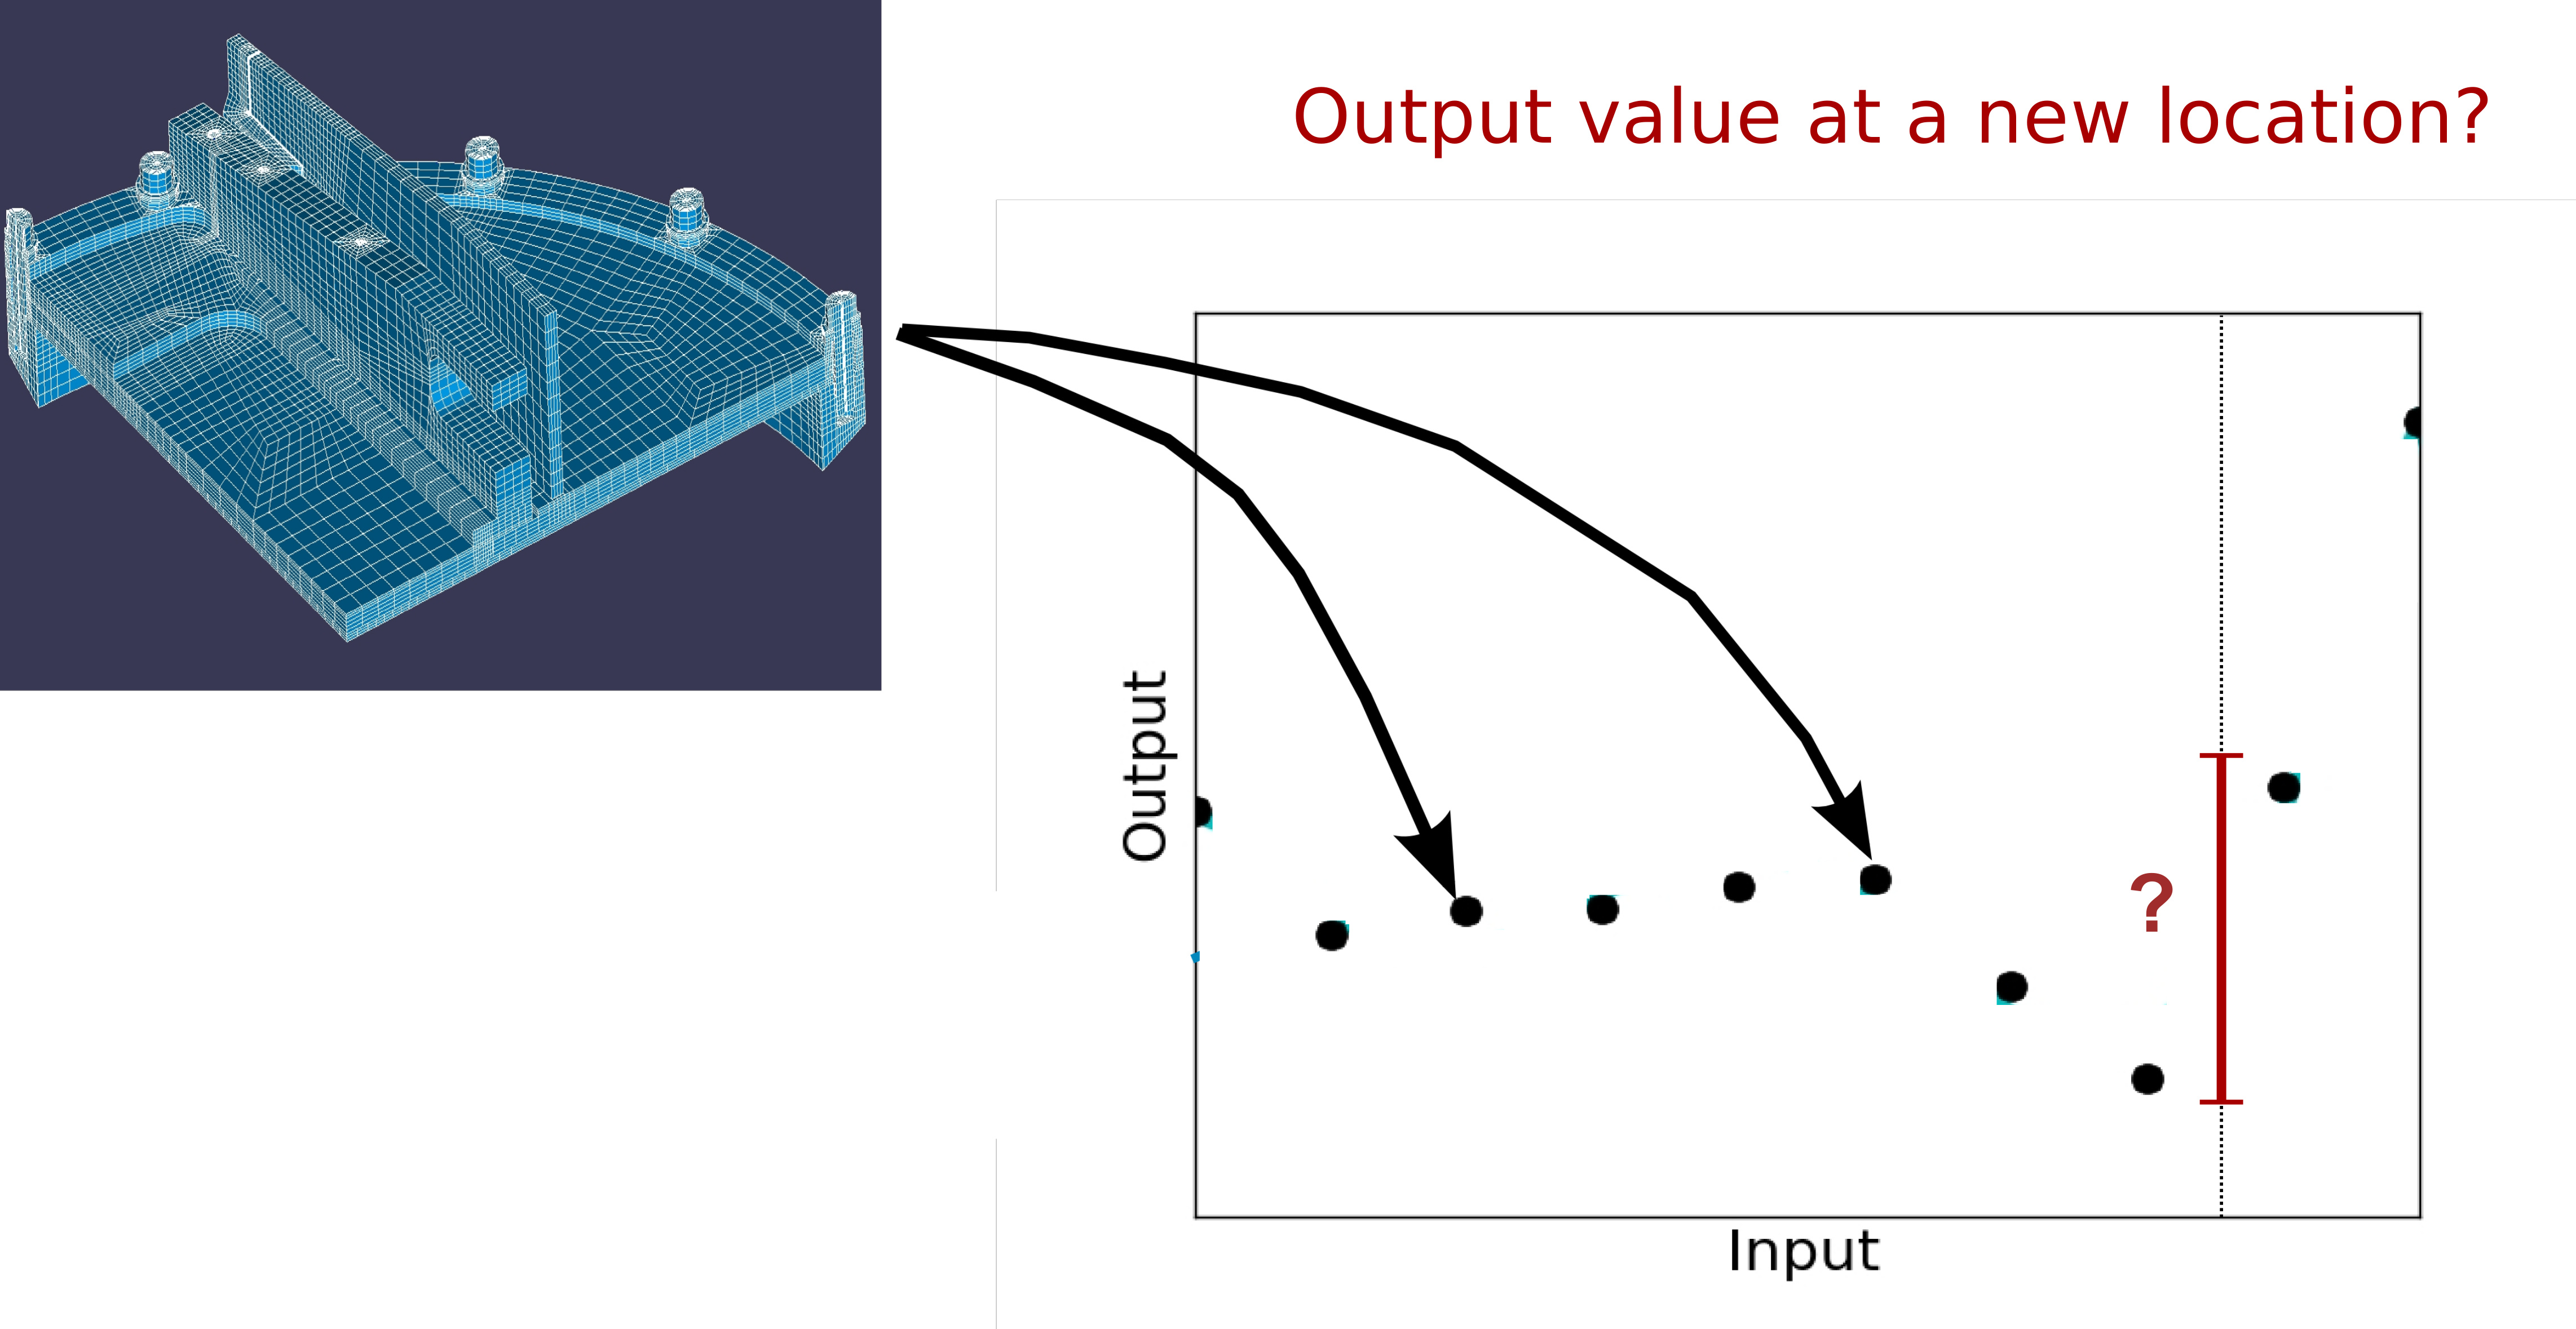
\includegraphics[width=9cm]{sketch-simu-new-loc.jpg} \\

\end{center}

\end{frame}

%=======================================================================================================%

\begin{frame}[t]{Prediction at a new point}

\begin{center}

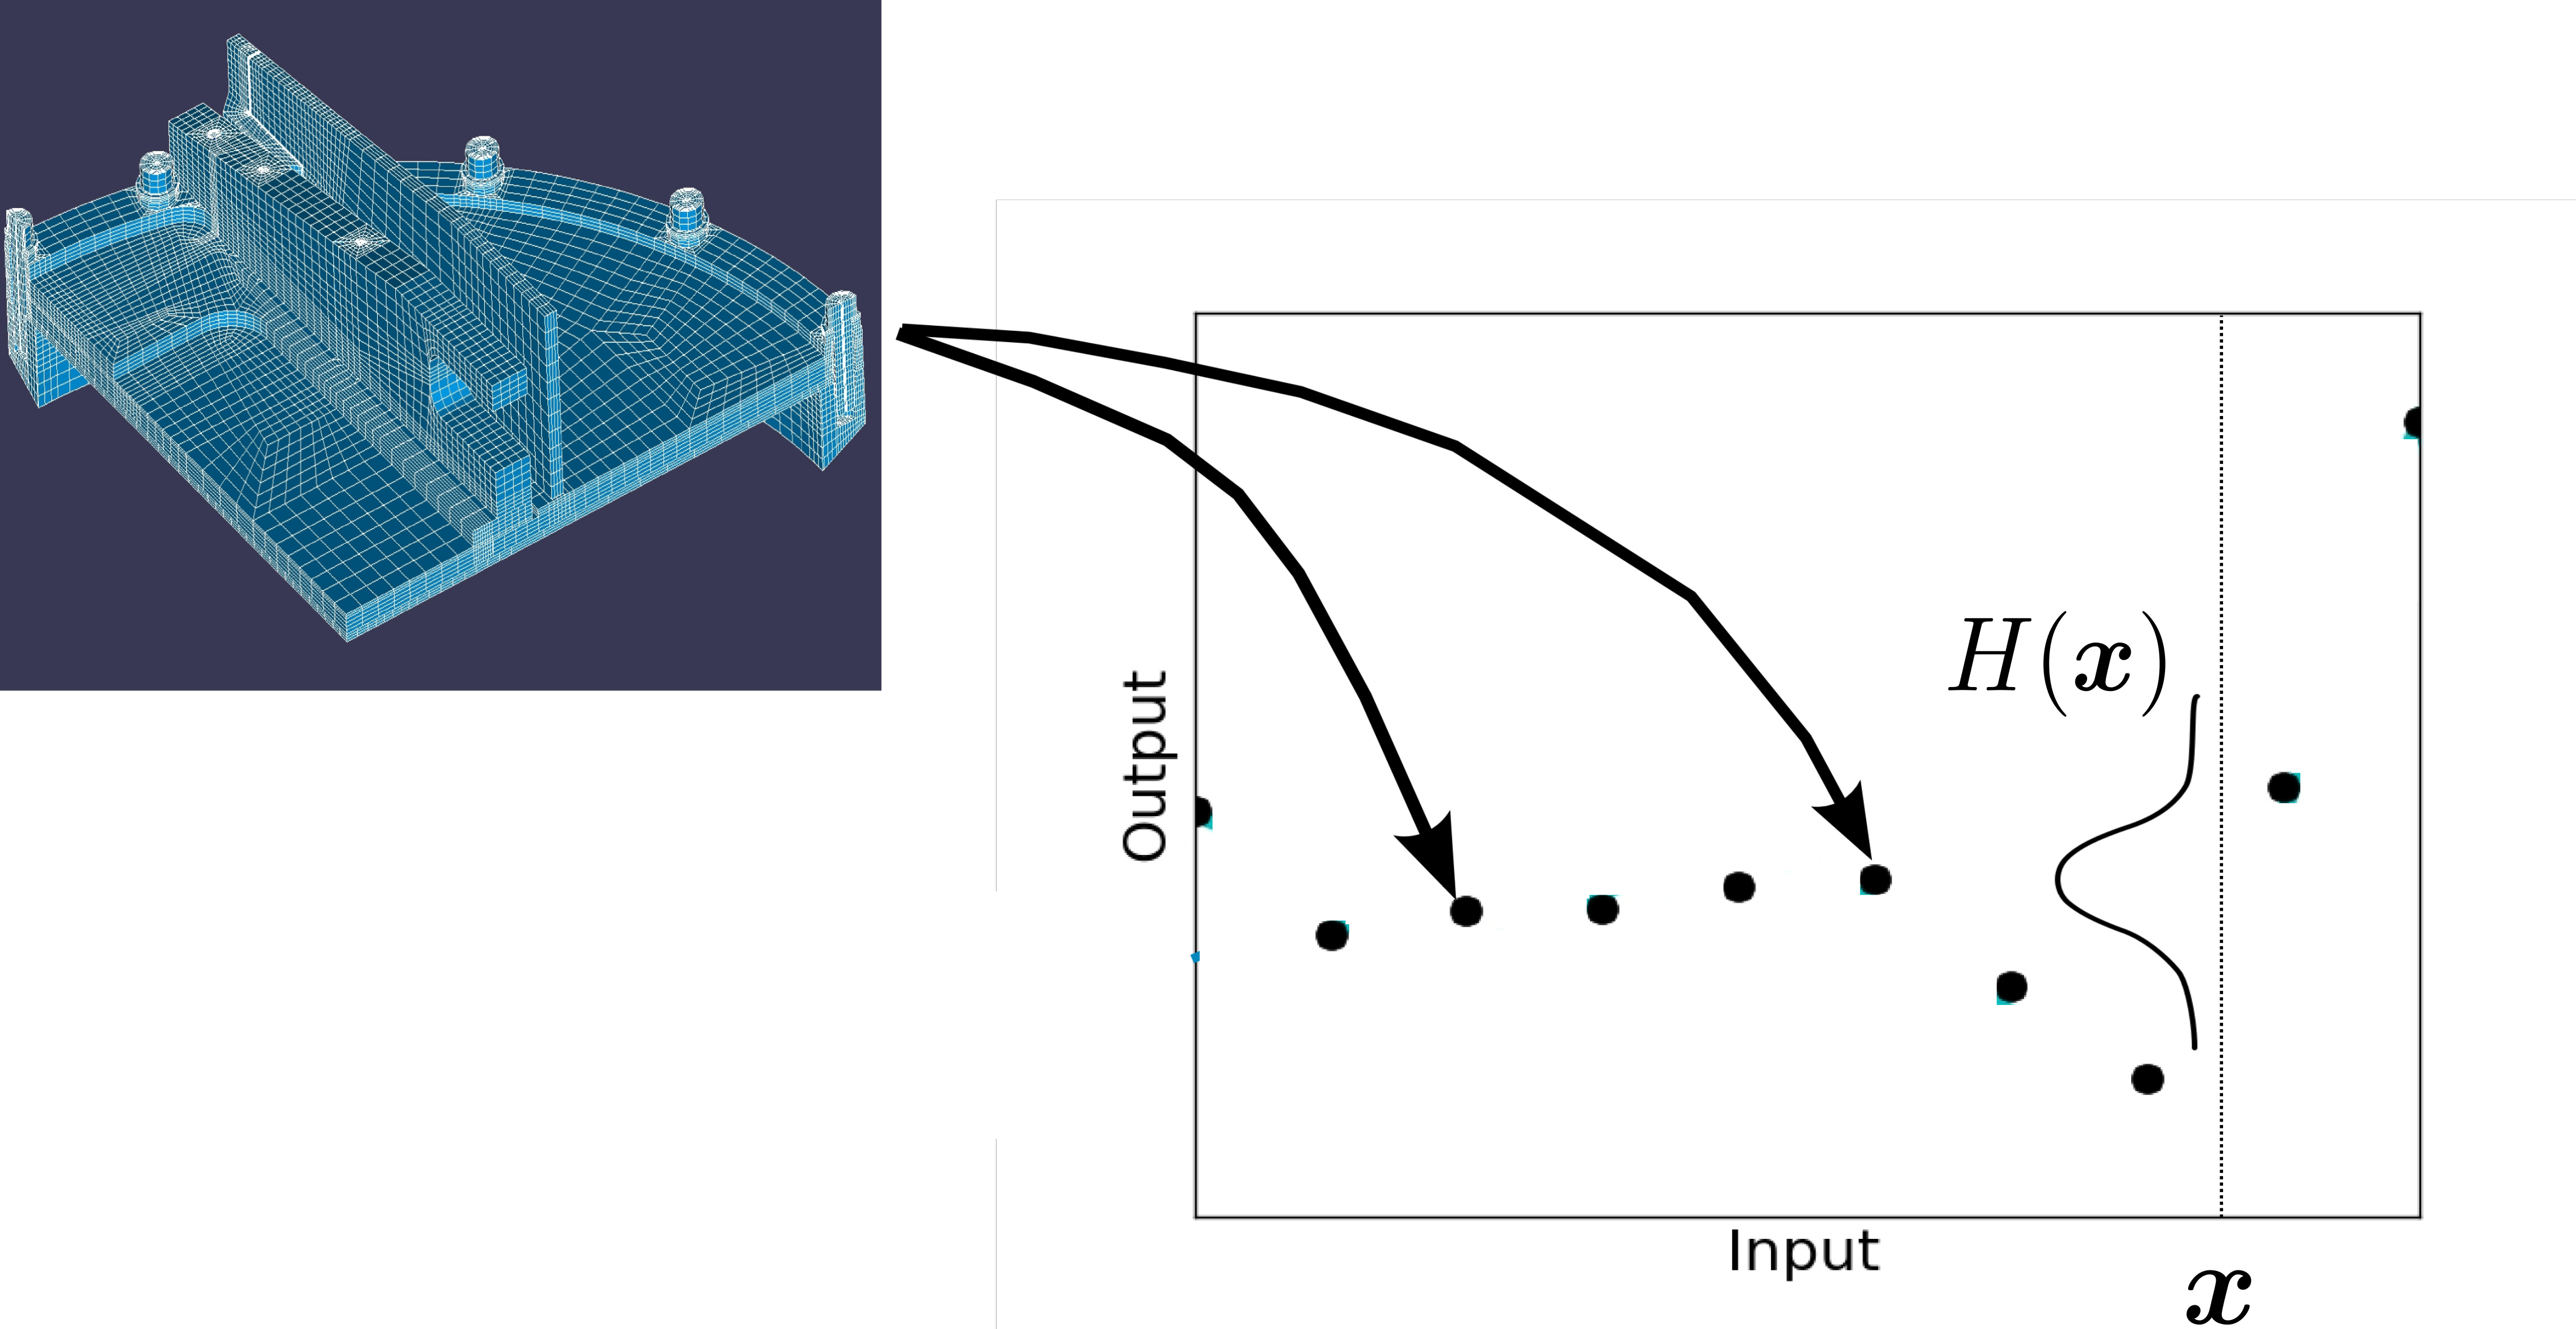
\includegraphics[width=9cm]{sketch-simu-new-loc-gaussian.jpg} \\

\end{center}

{{\bf Assumption:}~~The response is a realization of a {\altx Gaussian random variable} whose moments depend on the design points}

\end{frame}

%=======================================================================================================%

\begin{frame}{Gaussian process assumption}

The model output is a realization of a {\altx Gaussian random process} of the form~:

\vspace{0.3cm}

\begin{center}

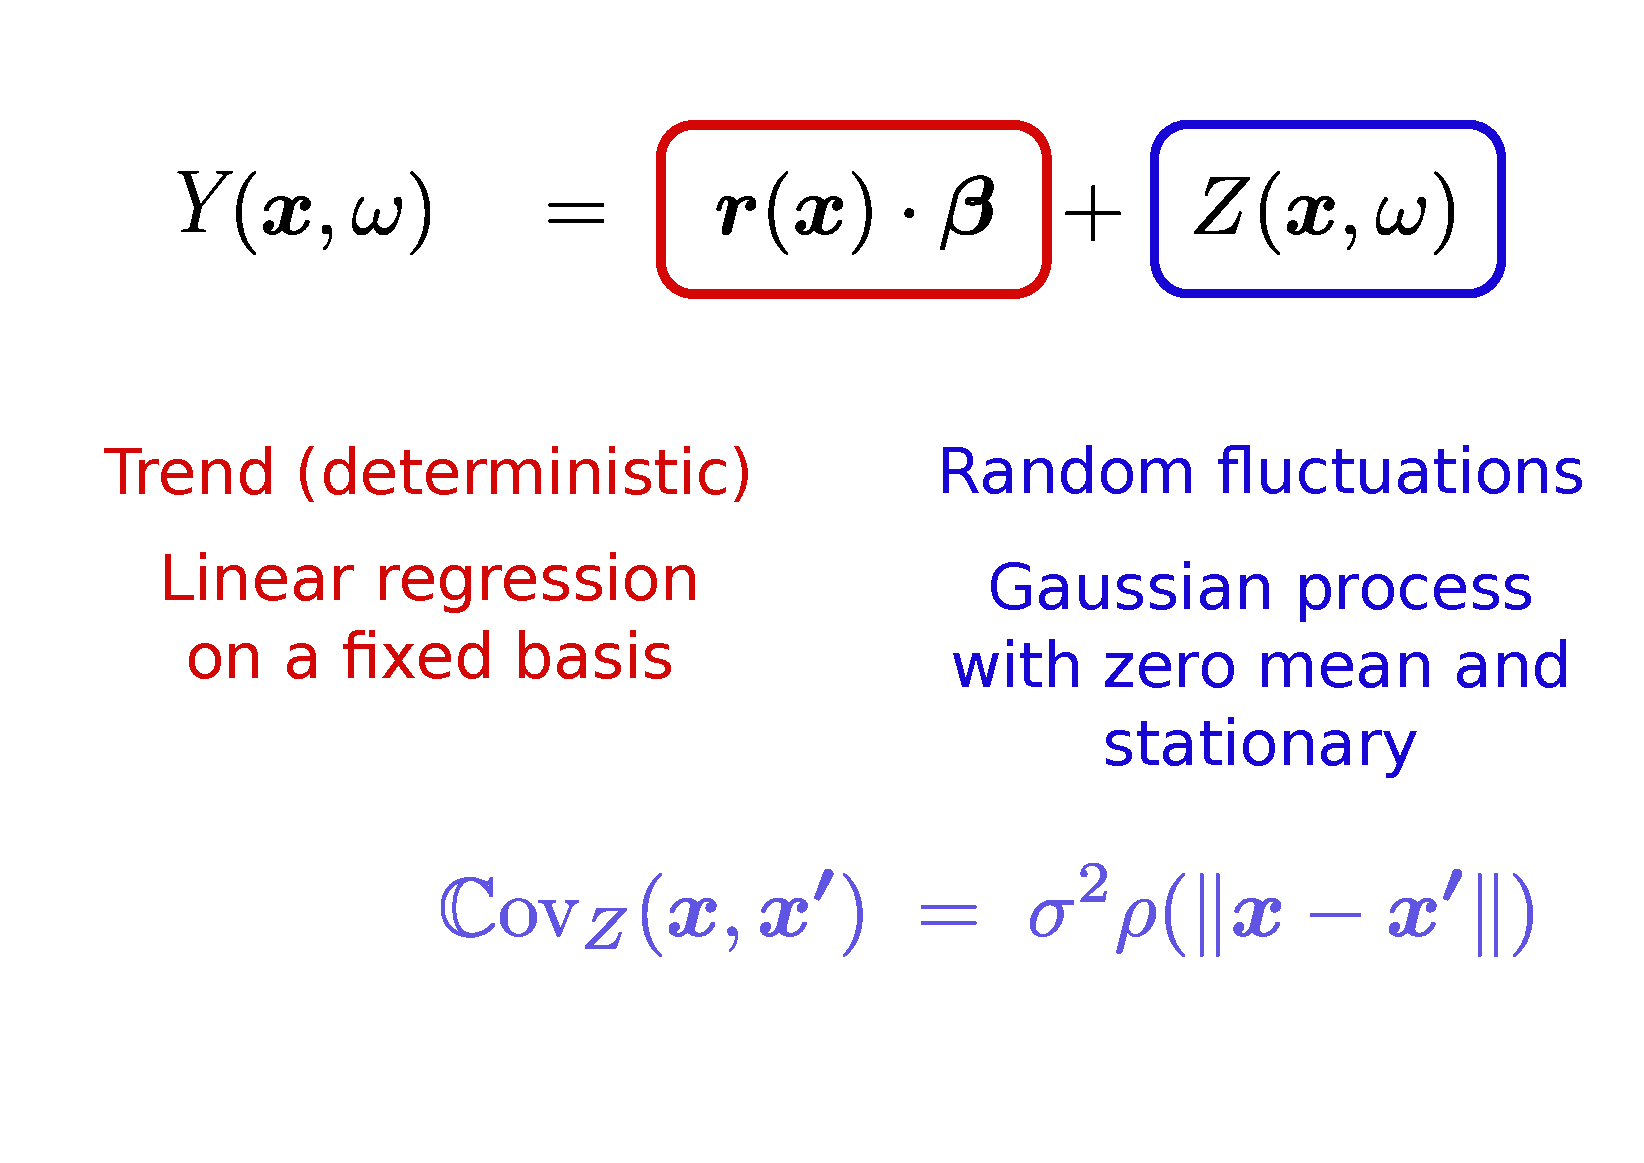
\includegraphics[width=7cm]{gp-equation-en.pdf} \\

{\altx \large Kriging}
\end{center}



\end{frame}

%=======================================================================================================%

\begin{frame}{Conditional mean and variance}

\begin{tabular}{ll}

{\altx Experimental design:}~~~ & $\mathcal{X} =  \left\{ \bs{x}^{(1)}, \dots ,  \bs{x}^{(N)}\right\} $ \\
& $\mathcal{Y} =  \left\{ Y(\bs{x}^{(1)}), \dots ,  Y(\bs{x}^{(N)}\right\} $\\
\\

{\altx Notations:}~~~ & $\bs{k}(\bs{x}) \, \, \equiv\, \, \left\{\rho\left(\bs{x},\bs{x}^{(1)}\right),\dots,\rho\left(\bs{x},\bs{x}^{(N)}\right)\right\}^{\tr}$ \\
 \\
& $\bs{R} \, \, \equiv\, \, \left( r_{j}(\bs{x}^{(i)}) \right)_{1\leq i,j\leq N} \quad , \quad \bs{K} \, \, \equiv\, \, \left( \rho(\bs{x}^{(i)},\bs{x}^{(j)}) \right)_{1\leq i,j\leq N}$ \\
\\
\\

{\altx Conditional mean:}~~~ & \fcolorbox{red}{white}{$\mu(\bs{x}) \, \, = \, \,   \bs{r}^{\tr}(\bs{x}) \bs{\beta} \, + \, \bs{k}^{\tr}(\bs{x}) \bs{K}^{-1} \left(\mathcal{Y} \, - \, \bs{R} \bs{\beta} \right)$} \\
\\
{\altx Conditional variance:}~~~ & \fcolorbox{red}{white}{$\sigma^{2}(\bs{x}) \, \, = \, \,   \sigma^{2} \, - \, \bs{k}^{\tr}(\bs{x}) \; \bs{K}^{-1} \; \bs{k}^{\tr}(\bs{x})$} \\
\end{tabular}
\end{frame}

%=======================================================================================================%

\begin{frame}{Conditional mean and variance}

Consider an instructive model: $y=f(x)=x\sin(x)$

Gaussian process metamodel:
\[ 
H(x,\omega) \; \; = \; \; \boldsymbol{r}(x) \cdot \boldsymbol{\beta} \; + \; Z(x,\omega) \qquad , \qquad 
\mathbb{C}\mbox{ov}_{Z}(x,x') \; \; = \; \; \sigma^2 e^{-\theta (x-x')^2}  
\]

\begin{center}
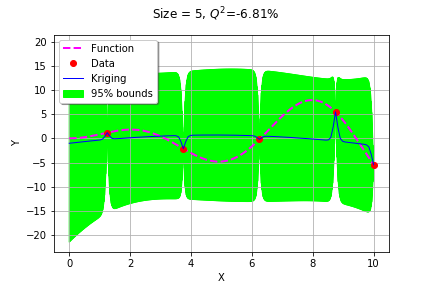
\includegraphics[width=0.49\linewidth]{krig_initial.png}
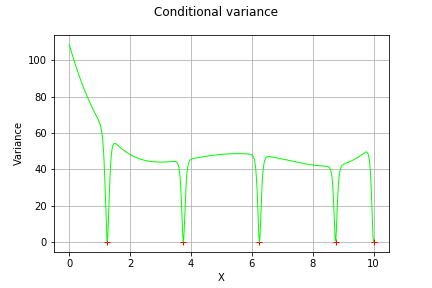
\includegraphics[width=0.49\linewidth]{var_initial.png}

\begin{itemize}
\item The conditional mean is used as a {\altx metamodel} (interpolator)
\item The conditional variance is used as an {\altx error indicator}
\end{itemize}

\end{center}

\end{frame}


%=======================================================================================================%

\begin{frame}{Parameter fitting}

To apply the previous formulas, the parameters $(\bs{\beta}, \sigma, \bs{\theta})$ have to be {\altx estimated} from the design points

\begin{itemize}
\item Optimal correlation parameter $\hat{\bs{\theta}}$ estimated by the {\altx maximum likelihood estimate} (Marrel et al. 2008) or {\altx cross validation} (Bachoc 2013)
\item Parameters $(\hat{\bs{\beta}}, \hat{\sigma})$ estimated by {\altx empirical best linear unbiased estimator} (BLUE) (Santner et al. 2003)

\end{itemize}

\end{frame}



%=======================================================================================================%
%
%\begin{frame}{Influence of the covariance function}
%
%\begin{center}
%
%\includegraphics[width=9cm]{sinus-func-gp-autocorr.pdf} \\
%
%The covariance function type has an effect on the metamodel
%
%\end{center}
%
%\end{frame}


%=======================================================================================================%

\begin{frame}{Sequential enrichment of the experimental design}

\begin{center}
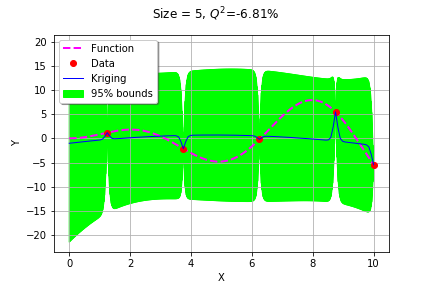
\includegraphics[width=0.6\linewidth]{krig_initial.png}\\
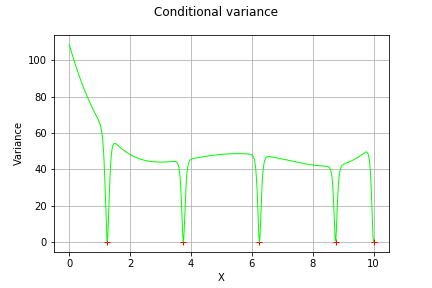
\includegraphics[width=0.6\linewidth]{var_initial.png}
\end{center}

\end{frame}

%=======================================================================================================%

\begin{frame}{Sequential enrichment of the experimental design}

\begin{center}
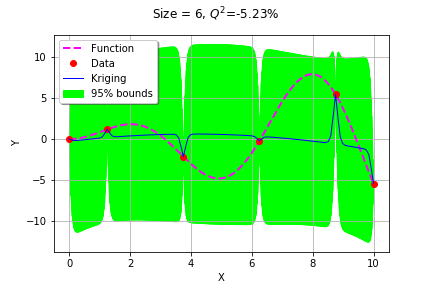
\includegraphics[width=0.6\linewidth]{krig_step_1.png}\\
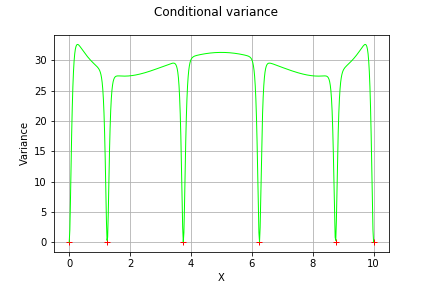
\includegraphics[width=0.6\linewidth]{var_step_1.png}
\end{center}

\end{frame}

%=======================================================================================================%

\begin{frame}{Sequential enrichment of the experimental design}

\begin{center}
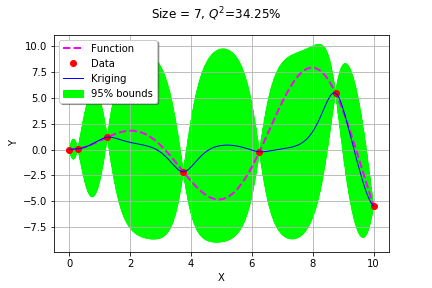
\includegraphics[width=0.6\linewidth]{krig_step_2.png}\\
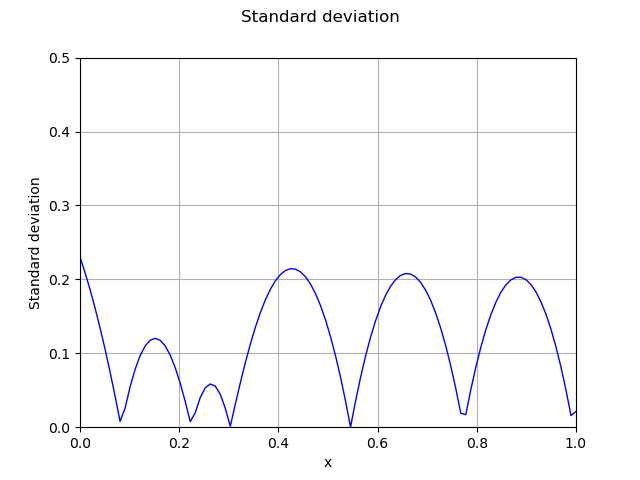
\includegraphics[width=0.6\linewidth]{var_step_2.png}
\end{center}

\end{frame}

%=======================================================================================================%

\begin{frame}{Sequential enrichment of the experimental design}

\begin{center}
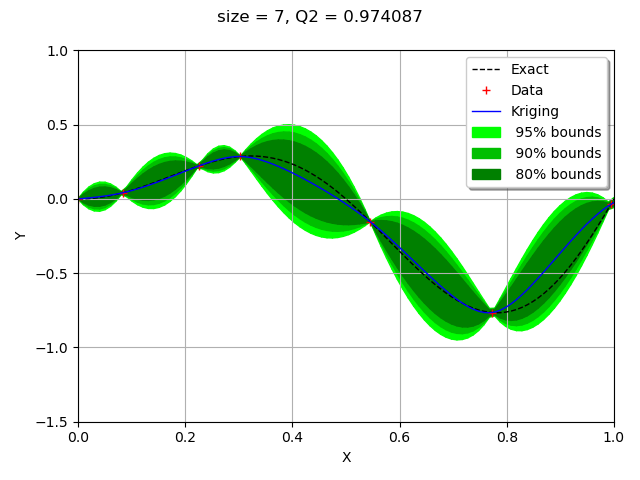
\includegraphics[width=0.6\linewidth]{krig_step_3.png}\\
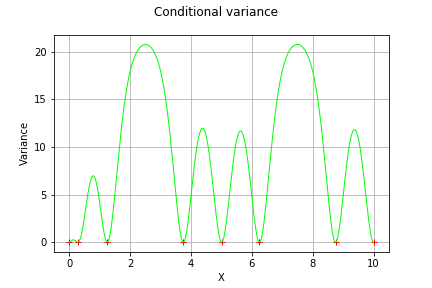
\includegraphics[width=0.6\linewidth]{var_step_3.png}
\end{center}

\end{frame}

%=======================================================================================================%

\begin{frame}{Sequential enrichment of the experimental design}

\begin{center}
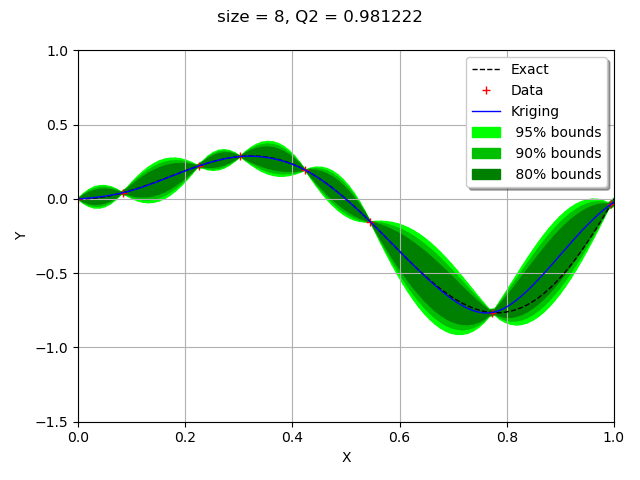
\includegraphics[width=0.6\linewidth]{krig_step_4.png}\\
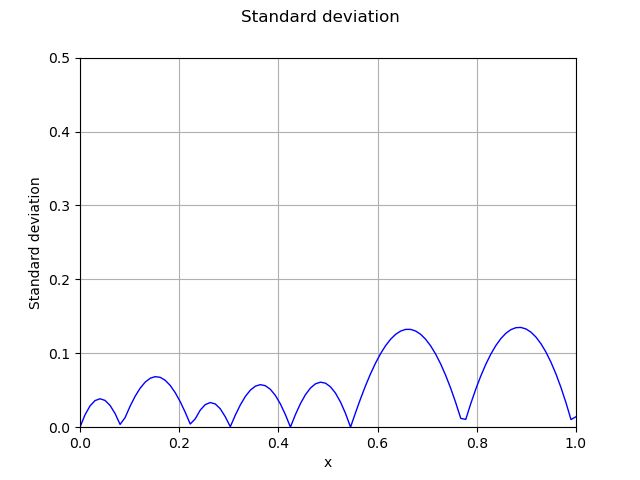
\includegraphics[width=0.6\linewidth]{var_step_4.png}
\end{center}

\end{frame}

%=======================================================================================================%

\begin{frame}{Sequential enrichment of the experimental design}

\begin{center}
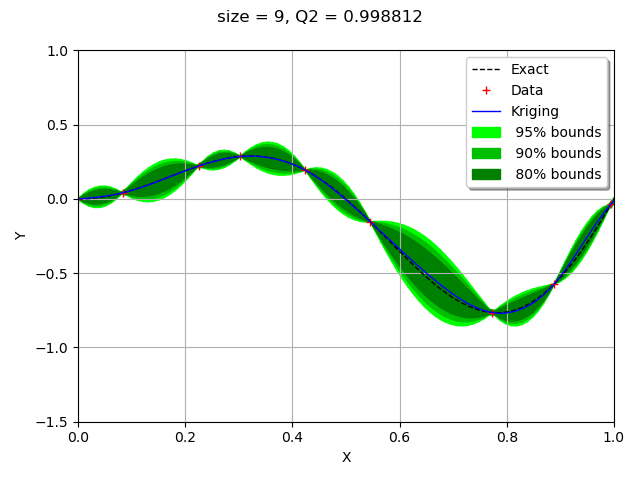
\includegraphics[width=0.6\linewidth]{krig_step_5.png}\\
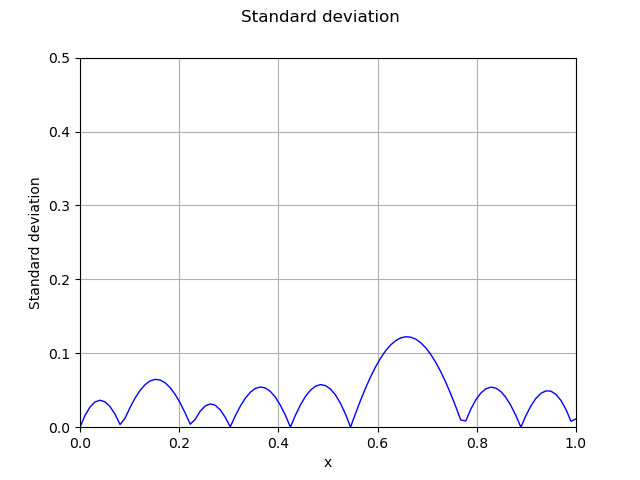
\includegraphics[width=0.6\linewidth]{var_step_5.png}
\end{center}

\end{frame}

\section{Conclusions}

\begin{frame}{Gaussian process metamodel }

\begin{itemize}
\item The regularity of the trajectories depends on the choice of covariance function
\vspace{0.6cm}
\item Kriging allows to associate a measure of certainty to a prediction of the function
\vspace{0.6cm}
\item Kriging allows the effective sequential enrichment of the experimental design
\end{itemize}

\end{frame}

\footnotesize

\pgfdeclareimage[height=1.0\paperheight, width=1.1\paperwidth]{end_image}{background_pages/end.pdf}
\setbeamertemplate{background canvas}{\pgfuseimage{end_image}}

\begin{frame}[plain]
		\vskip-3ex
\begin{columns}[t]
	\begin{column}{5.5cm}
  \begin{center}
  \textcolor{orange}{\Huge Thank you}
  \end{center}
  	\end{column}
	\begin{column}{3.2cm}
	  	\end{column}
	  	\end{columns}
\end{frame}

\end{document}
